The number of responses to each question may vary as none of the questions are mandatory in our survey (to encourage a higher response rate). Hence, not all participants answered all questions. 
Figure \ref{fig:developers_experience_in_general} shows the participants' experience in software development. 
We collect the data in Figure~\ref{fig:developers_experience_in_general} from \textit{Question \#3} where the options range from ``0 years'' to ``10 or more years''. We observe that 78\% (\nicefrac{348}{444}) of participants have eight or more years of experience in software development. 
Finally, Figure \ref{fig:developers_experience_using_ci} shows the experience of participants with CI. 64.2\% (\nicefrac{282}{439}) of participants have five or more years of experience with CI. Only five (1.3\%) participants report less than one year of experience with CI. 

\begin{figure}[H]
	\centering
	\begin{subfigure}[b]{0.3\textwidth}
		\centering
		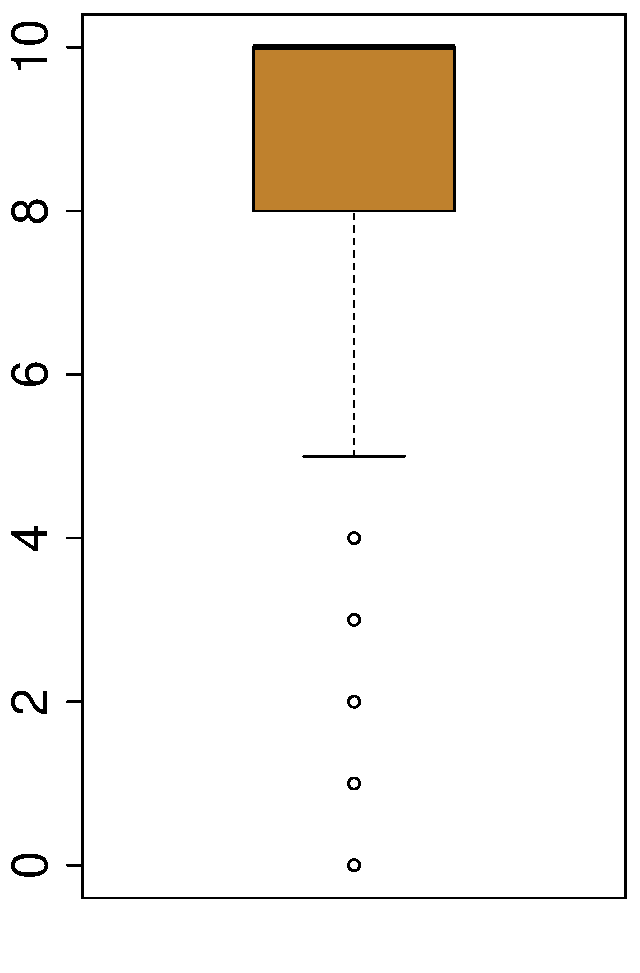
\includegraphics[width=2.7cm, height=4.0cm]{developer_experience_in_general.pdf}
		\caption{In general.}
		\label{fig:developers_experience_in_general}
	\end{subfigure} %
%	\begin{subfigure}[b]{0.3\textwidth}
%		\centering
%		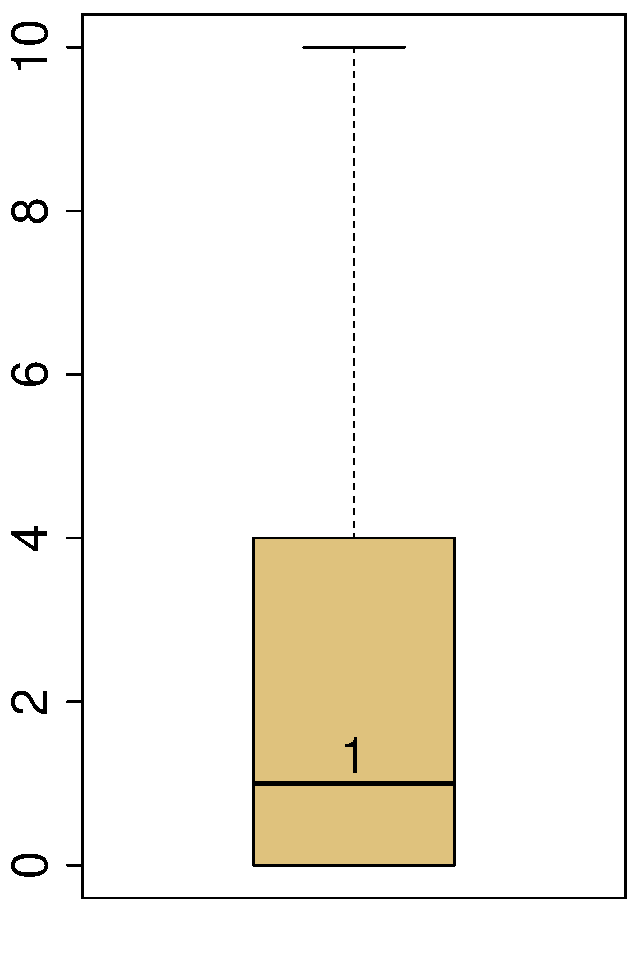
\includegraphics[width=2.5cm, height=4.0cm]{./images/developer_experience_on_the_studied_project.pdf}
%		\caption{On the studied project.}
%		\label{fig:developers_experience_on_the_studied_project}
%	\end{subfigure}
	\begin{subfigure}[b]{0.3\textwidth}
		\centering
		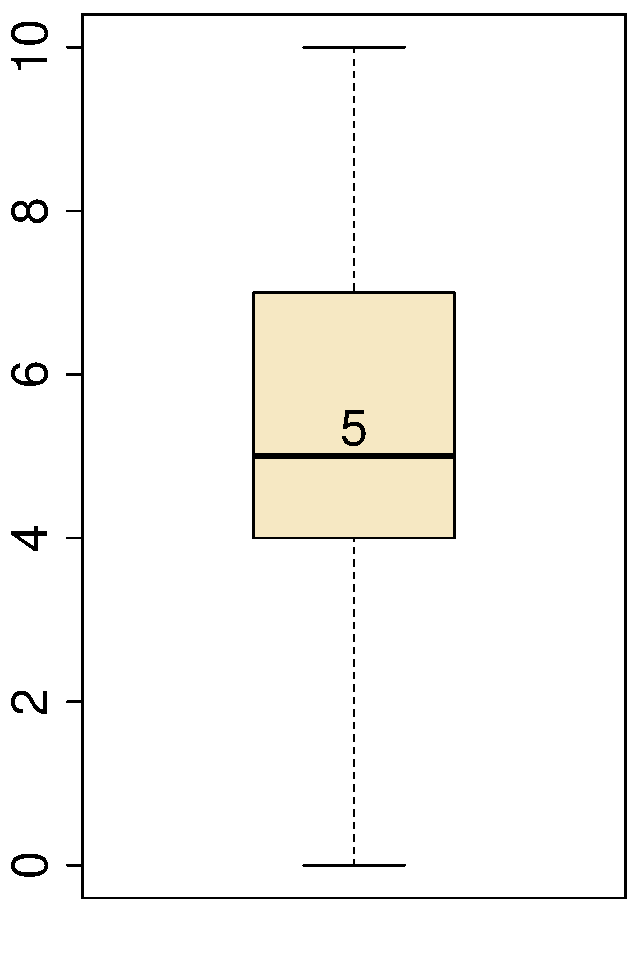
\includegraphics[width=2.5cm, height=4.0cm]{developer_experience_using_CI.pdf}  
		\caption{Using CI.}
		\label{fig:developers_experience_using_ci}
	\end{subfigure}
	\caption{Participants' experience in software development.}
	\label{fig:developers_experience}
\end{figure}

We observe that 51.8\% (\nicefrac{226}{436}) of participants used CI in 60--100\% of their projects (see Figure \ref{fig:ratio_of_projects_using_ci}). 
%Lastly, 26.8\% (\nicefrac{117}{436}) of our participants report that a ratio of 0--40\%  of the projects they have worked on use CI 
In terms of participants' main activities, we observe that the development of new features is the most common activity among them, followed by test and review. A total of 92.9\% of participants state that developing new features is one of their main activities in their projects. Another 229 participants (50.9\%) state that code review is another main activity they perform in their projects. Figure \ref{fig:main_development_activities} shows the participants' main activities according to their own classification (\textit{Question \#7}). Given that a participant can take on several roles, the sum of the percentages in Figure \ref{fig:main_development_activities} can be greater than 100\%.
%which can help us identify whether the perceived influence of CI on the delivery time of merged PRs can be associated with certain profiles
Considering the demographics, we were able to collect a diverse set of participants in terms of experience with CI, domain area, and development activities (e.g., bug fixing, developing new features, or code review). 

\begin{figure}[!t]
	\centering
	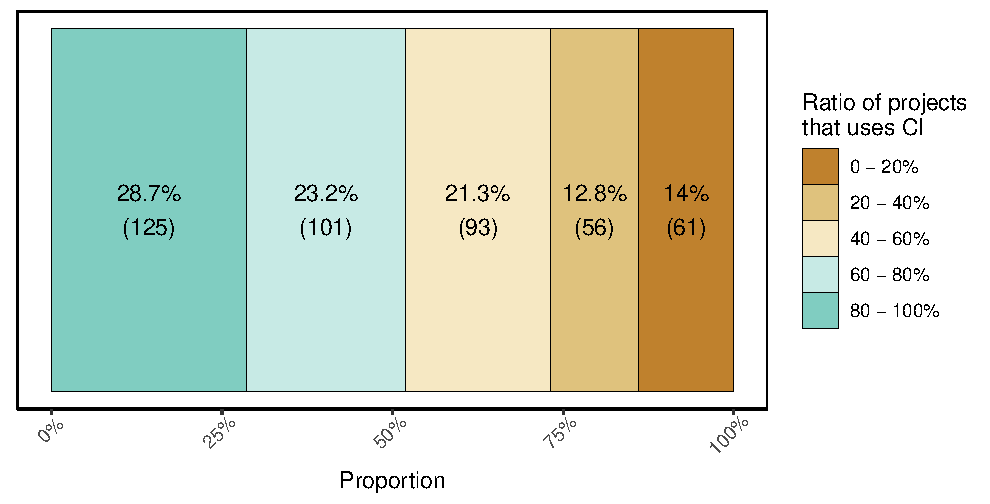
\includegraphics[ width=9cm]{ratio_of_projects_using_ci.pdf}
	% figure caption is below the figure
	\caption{Proportion of participants' projects that use CI (\textit{Question \#5}).}
	\label{fig:ratio_of_projects_using_ci}       % Give a unique label
\end{figure}

\begin{figure}[H]
	\centering
	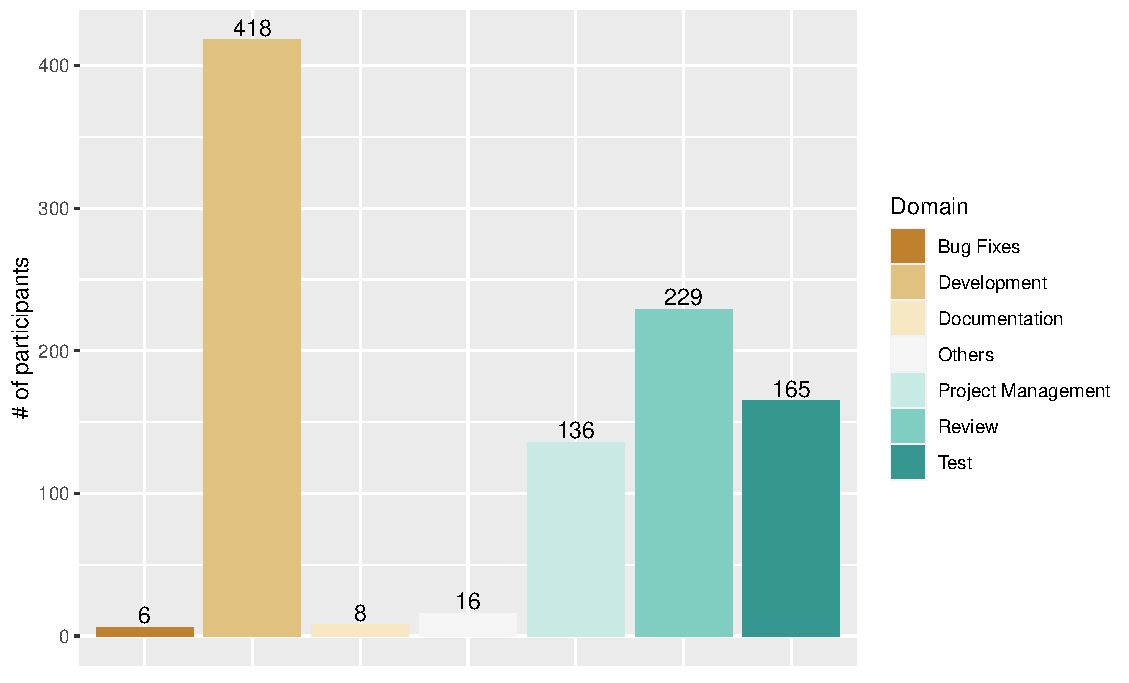
\includegraphics[ width=10cm]{main_development_activities.pdf}
	% figure caption is below the figure
	\caption{Developers' main activities.}
	\label{fig:main_development_activities}       % Give a unique label
\end{figure}

With respect to {\em domain expertise}, we observe that {\em web development} is the most common domain of our participants. 77.8\% (\nicefrac{350}{450}) of participants state that web development is one of their main domains (\textit{Question \#8}). The second and third most common domains are business software development (35.3\%, \nicefrac{159}{450}) and mobile applications (32.2\%, \nicefrac{145}{450}). 
Business software is a system used to measure and improve enterprise productivity and to perform other business functions. Document Management Systems, Employee Scheduling Software, and Enterprise Resource Planning (ERP) are examples of business software. Additionally, a significant number of participants are from areas such as scientific development (i.e., those who develop software systems to analyze, visualize, or simulate processes or data) and big data (i.e., those who use scientific software to process and analyze data). This diversity of domains demonstrates that we obtain insights from several roles and development areas.

\begin{figure}[H]
	\centering
	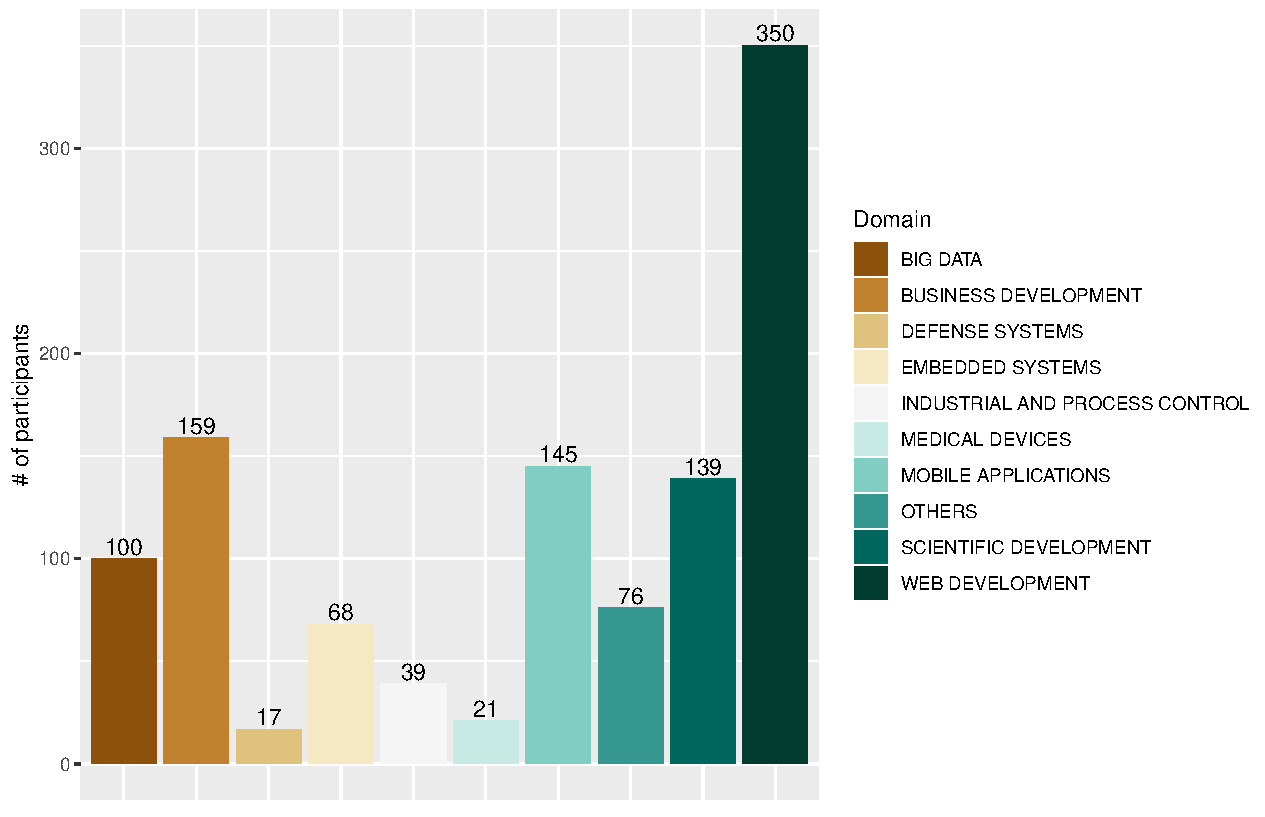
\includegraphics[ width=10cm]{developer_domain_area.pdf}
	% figure caption is below the figure
	\caption{Participants' domain area.}
	\label{fig:developer_domain_area}       % Give a unique label
\end{figure}

In Table \ref{tab:themes_per_research_question} we present the summary of Themes that were generated by our thematic analysis for each research question (RQ). 
For instance, in $RQ4$ we investigate the perceived influence of CI on the delivery time of merged PRs, which is associated with the following themes: \textit{automation}, \textit{project quality}, and \textit{release process}. 
Additionally, a theme may emerge in the results of more than one RQ. For instance, the \textit{automation} theme emerges in the results of both $RQ4$ and $RQ6$. This is because participants of our study believe that \textit{automation} impacts the delivery time of merged PRs ($RQ4$) while also impacting the release process of projects ($RQ6$). Table \ref{tab:themes_per_research_question} presents an overview of the findings of the qualitative study. The detailed analysis for each theme is described in the result section of $RQ4$---$RQ8$.

% Table generated by Excel2LaTeX from sheet 'Themes per RQ'
\begin{table}
	\centering
	\caption{High-level Overview of the Themes per RQ of the qualitative study.}
% Table generated by Excel2LaTeX from sheet 'Themes per RQ'
    \begin{tabular}{cp{15em}}
    \hline
    \textbf{Research Question} & \multicolumn{1}{c}{\textbf{Theme}} \bigstrut\\
    \hline
    \multicolumn{1}{l}{\multirow{3}[6]{*}{\textbf{RQ4:} Impact of CI on the PR delivery time}} & \multicolumn{1}{l}{Automation} \bigstrut\\
    \cline{2-2}          & \multicolumn{1}{l}{Project quality} \bigstrut\\
    \cline{2-2}          & Release process \bigstrut\\
    \hline
    \multicolumn{1}{l}{\multirow{6}[13]{*}{\textbf{RQ5:} Themes that impact the PR delivery time in general}} & \multicolumn{1}{l}{PR characteristics} \bigstrut\\
\cline{2-2}          & \multicolumn{1}{l}{Project maintenance} \bigstrut\\
\cline{2-2}          & \multicolumn{1}{l}{Release process} \bigstrut\\
\cline{2-2}          & \multicolumn{1}{l}{Team characteristics} \bigstrut\\
\cline{2-2}          & \multicolumn{1}{l}{Contributors} \bigstrut\\
\cline{2-2}          & \multicolumn{1}{l}{Testing} \bigstrut\\
    \hline
    \multicolumn{1}{l}{\multirow{3}[6]{*}{\textbf{RQ6:} Influence of CI on the project release process}} & Automation \bigstrut\\
\cline{2-2}          & Project Stability \bigstrut\\
\cline{2-2}          & Release characteristics \bigstrut\\
    \hline
    \multicolumn{1}{l}{\multirow{2}[4]{*}{\textbf{RQ7:} Influence of CI on the project review process}} & CI does not impact code review \bigstrut\\
\cline{2-2}          & CI impacts code review \bigstrut\\
    \hline
    \multicolumn{1}{l}{\multirow{2}[4]{*}{\textbf{RQ8:} Impact of CI on attracting more contributors}} & Attractive project characteristics \bigstrut\\
\cline{2-2}          & Lower contribution barrier \bigstrut\\
    \hline
    \end{tabular}%
  \label{tab:themes_per_research_question}%
\end{table}%